\documentclass{ctexart}[UTF8]
\usepackage{dirtree}
\usepackage{listings}
\usepackage{xcolor}
\usepackage{graphicx}
\usepackage{enumerate}
\usepackage[a4paper]{geometry} 
\usepackage{amsmath,amsthm,mathtools,amssymb}
\usepackage{mathtools}
\usepackage{diagbox}
\usepackage{multirow,makecell}
\usepackage{float}
\usepackage{url}
\usepackage[nottoc]{tocbibind}
\usepackage{float}
\newcommand{\refe}[1]{Eq.\ref{#1}}
\newcommand{\reft}[1]{Theory.\ref{#1}\ }
\newcommand{\reff}[1]{图\ref{#1}\ }
\lstset{
 columns=fixed,
 numbers=left,                                        % 在左侧显示行号
 numberstyle=\tiny\color{gray},                       % 设定行号格式
 basicstyle=\small\ttfamily,
 frame=none,                                          % 不显示背景边框
 backgroundcolor=\color[RGB]{245,245,244},            % 设定背景颜色
 keywordstyle=\color[RGB]{40,40,255},                 % 设定关键字颜色
 numberstyle=\footnotesize\color{darkgray},           
 commentstyle=\color{gray}\ttfamily,                  % 设置代码注释的格式
 stringstyle=\rmfamily\slshape\color[RGB]{128,0,0},   % 设置字符串格式
 showstringspaces=false,
 breaklines=true,
 language=c++
}
\newtheorem{theorem}{Theory}[section]
\geometry{bottom=2cm,left=1cm,right=1cm}
\author{张配天-2018202180}
\title{上机6}
\begin{document}
    \maketitle
    \tableofcontents
    \clearpage
    \section{问题描述}
    输入$m$个数,使用最坏情况为线性时间的算法选择出第$k$小的数。
    \subsection{输入}
    5000个不重复数构成的数组,以及$k$;
    \subsection{输出}
    第$k$小的数;
    \section{算法思路}
    \begin{enumerate}
        \item 分别定义select函数和partition函数
        \item 将输入的数组分为$\lceil n/5 \rceil$组,每组进行插入排序,找到中位数后\textbf{将中位数移到数组最前端}
        \item 递归调用select函数选出中位数的中位数所在的位置$l$,再调用partition函数将比中位数的中位数小的元素放在左边,比中位数大的元素放在右边;select函数的递归边界是数组仅有一个元素时,直接返回自身下标
        \item 判断要找的第$k$小的元素是不是中位数的中位数所在的位置,如果$k<l$ ,则从前面一半的数组递归调用select函数找第$k$小的元素;如果$k>l$,则从后面一半的数组递归调用select函数找第$l-k$小的元素    
    \end{enumerate}
    \section{复杂度分析}
    \subsection{细节分析}
    \begin{enumerate}
        \item 首先分组排序,$O(n)$:\begin{figure}[H]
            \centering
            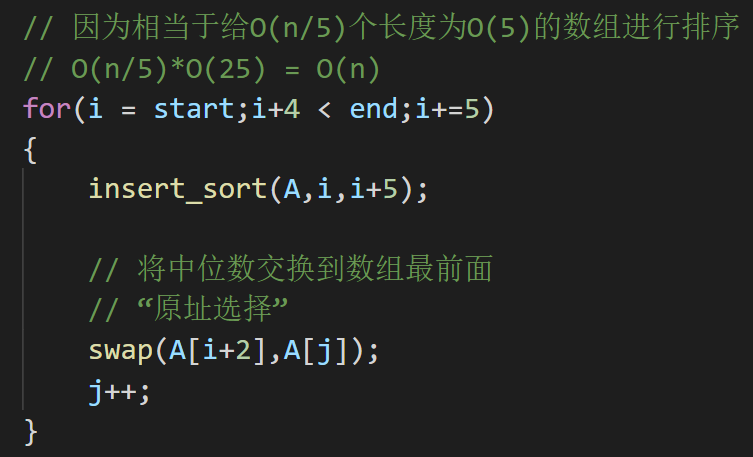
\includegraphics[width=10cm]{../Resources/6_2.png}
        \end{figure}
        \item 之后递归找中位数,$T(\left\lceil \frac{n}{5}\right\rceil)$:\begin{figure}[H]
            \centering
            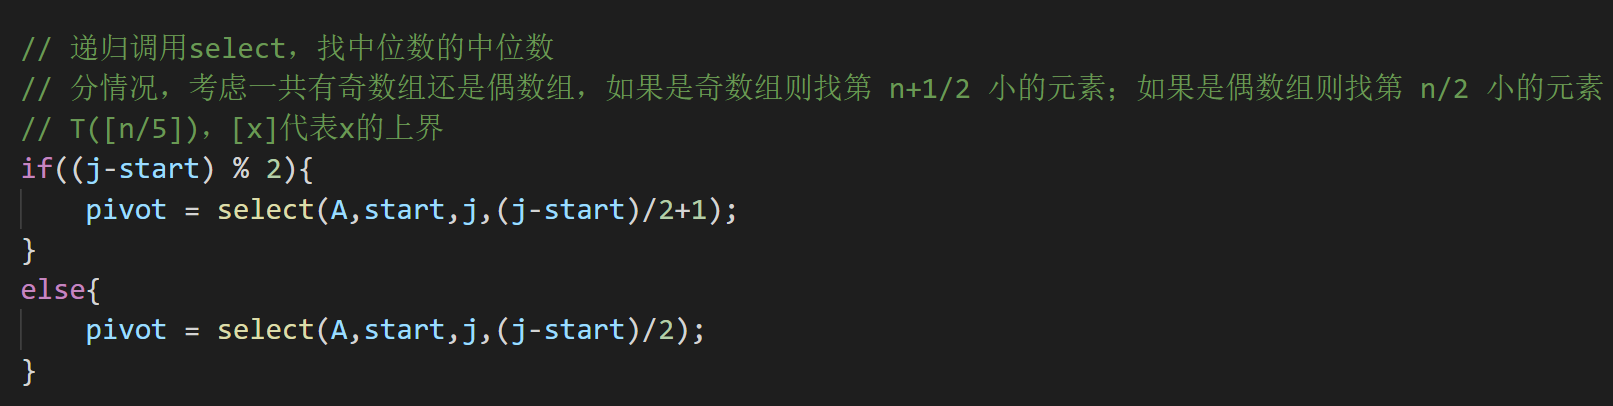
\includegraphics[width=10cm]{../Resources/6_3.png}
        \end{figure}
        \item 最后递归找位置$T(\frac{7n}{10} + 6)$:\begin{figure}[H]
            \centering
            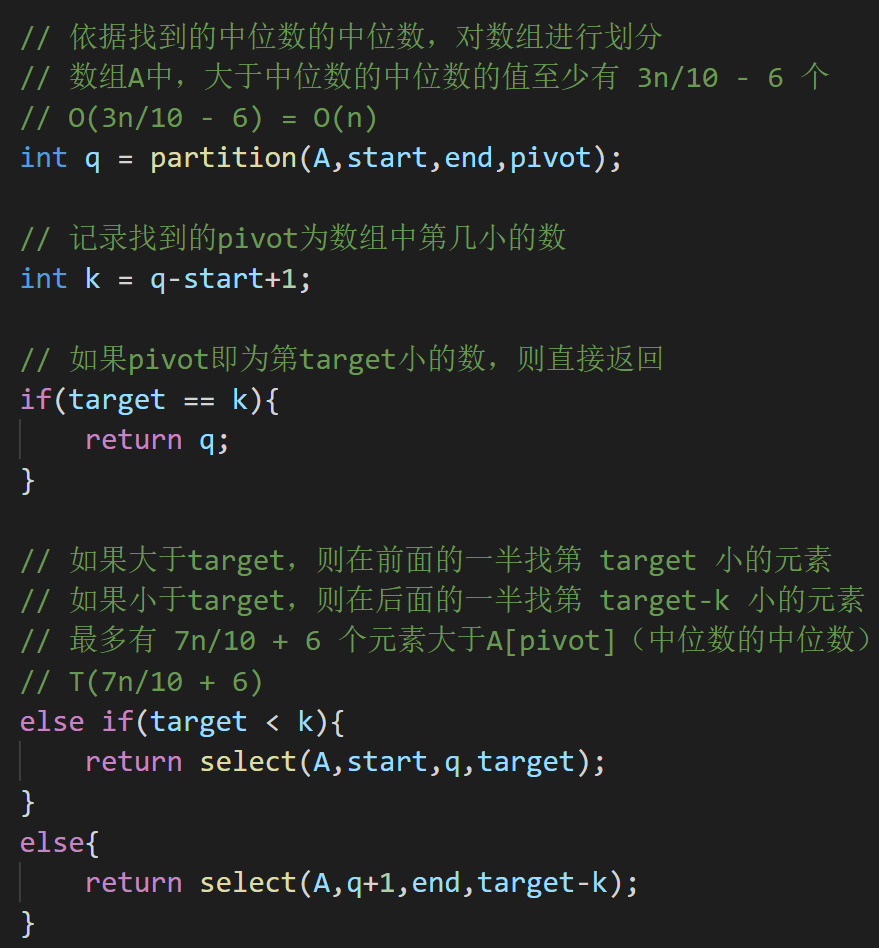
\includegraphics[width=10cm]{../Resources/6_4.png}
        \end{figure}

    \end{enumerate}
    % 2. 之后递归找中位数,$T(\left\lceil \frac{n}{5}\right\rceil)$![](../Resources/6_3.png)
    % 3. 最后递归找位置$T(\frac{7n}{10} + 6)$![](../Resources/6_4.png)
    \subsection{证明最差为线性时间复杂度}
    经过分析,有时间复杂度如下:
    \begin{align}
        T(n) = 
            O(n) + T(\frac{7n}{10} + 6) + T( \left\lceil\frac{n}{5} \right\rceil) & n \ge 140\\
            O(1)&n< 140
    \end{align}
    利用代入法:假设存在$n_0\in \mathbb{N}^+,c\in \mathbb{R}$,使得当$n\ge n_0$ 时很有$T(n) \leq cn$,同时有$a\in \mathbb{R}\ s.t.\ O(n) \leq an$则有:
    \begin{equation}
        T(n) \leq an + c(\frac{7n}{10} + \left\lceil \frac{n}{5}\right\rceil ) \leq an + \frac{7cn}{10} + 6c + \frac{cn}{5} + c
    \end{equation}
    则有
    \begin{equation}
        T(n) \leq \frac{9cn}{10} + 7c + an = cn + (-\frac{cn}{10} + 7c + an)
    \end{equation}
    我们令
    \begin{equation}
        -\frac{cn}{10} + 7c + an <= 0\ \implies c\ge \frac{10an}{n-70}
    \end{equation}
    假设$n\ge 140(n_0 = 140)$,则有$c\ge 20a$;考虑初始情况:$O(1) \leq cn_0$,因此$T(n) = O(n)$得证。
    \section{源代码}
    \begin{lstlisting}
#include<fstream>
#include<iostream>
#include<limits.h>
using namespace std;
// 定义输出数组的函数,方便调试
void print(int * a,int length){
    for(int i = 0;i < length;i++){
        cout<<a[i]<<endl;
    }
    return;
}

// 插入排序
// O((end-start)^2)
void insert_sort(int *A,int start,int end){
    
    int i = start+1;
    while(i < end){
        int v = *(A+i);
        int j = i-1;
        while(*(A+j) > v && j >= start){
            *(A+j+1) = *(A+j);
            j--; 
        }
        *(A+j+1) = v;
        i++;
    }
}

// 划分
// 将小于等于A[pivot]的值都放在其左边,大于的放在右边
int partition(int *A,int start,int end,int pivot){
    int x = A[pivot];
    
    // 首先将A[pivot]换到数组末尾,防止在交换过程中被调换了位置
    // O(1)
    swap(A[pivot],A[end-1]);
    int i = start-1;

    // 进行排序
    // O((end-start)^2)
    for(int j = start;j < end-1;j++){
        if(A[j] <= x){
            i++;
            swap(A[i],A[j]);
        }
    }
    swap(A[i+1],A[end-1]);
    return i+1;
}

// 选择函数
// 从A[start:end]中选出第target小的数的索引
int select(int *A,int start,int end,int target){
    // 如果数组长度为1,则直接返回
    if(end-start == 1) return start;

    // 初始复制
    // O(1)
    int i = 0,j = start;
    int length = end-start;
    int remain = length%5;

    // 因为相当于给O(n/5)个长度为O(5)的数组进行排序
    // O(n/5)*O(25) = O(n)
    for(i = start;i+4 < end;i+=5)
    {
        insert_sort(A,i,i+5);

        // 将中位数交换到数组最前面
        // “原址选择”
        swap(A[i+2],A[j]);
        j++;
    }

    // 如果有不能被5整除的部分,则单独划为一组
    // O(25)
    if(remain){
        insert_sort(A,end-remain,end);

        // 将中位数交换到数组最前面
        // “原址选择”
        swap(A[j],A[end-remain/2-1]);
        j++;
    }

    int pivot = 0;

    // 递归调用select,找中位数的中位数
    // 分情况,考虑一共有奇数组还是偶数组,如果是奇数组则找第 n+1/2 小的元素;如果是偶数组则找第 n/2 小的元素
    // T([n/5]),[x]代表x的上界
    if((j-start) % 2){
        pivot = select(A,start,j,(j-start)/2+1);
    }
    else{
        pivot = select(A,start,j,(j-start)/2);
    }
    
    // 依据找到的中位数的中位数,对数组进行划分
    // 数组A中,大于中位数的中位数的值至少有 3n/10 - 6 个
    // O(3n/10 - 6) = O(n)
    int q = partition(A,start,end,pivot);

    // 记录找到的pivot为数组中第几小的数
    int k = q-start+1;

    // 如果pivot即为第target小的数,则直接返回
    if(target == k){
        return q;
    }

    // 如果大于target,则在前面的一半找第 target 小的元素
    // 如果小于target,则在后面的一半找第 target-k 小的元素
    // 最多有 7n/10 + 6 个元素大于A[pivot](中位数的中位数)
    // T(7n/10 + 6)
    else if(target < k){
        return select(A,start,q,target);
    }
    else{
        return select(A,q+1,end,target-k);
    }
}

int main(){
    int A[5000];
    int i = 0,j = 0;
    string value;

    // 读入文件
    ifstream fin("D:\\Data\\Class_data\\Alg_data\\lab4.txt");
    for(int i=0;i<5000;i++)
		fin>>A[i];

    cout<<"which ORDER statistic you want to find?"<<endl;
    cin>>j;
    int result = select(A,0,5000,j);
    cout<<j<<"th smallest number is: "<<A[result]<<endl;

    // 可以使用下面的测试
    // insert_sort(A,0,5000);
    // cout<<A[999];
    
    return 0;
}
    \end{lstlisting}
    \section{运行截图}
        \begin{figure}[H]
            \centering
            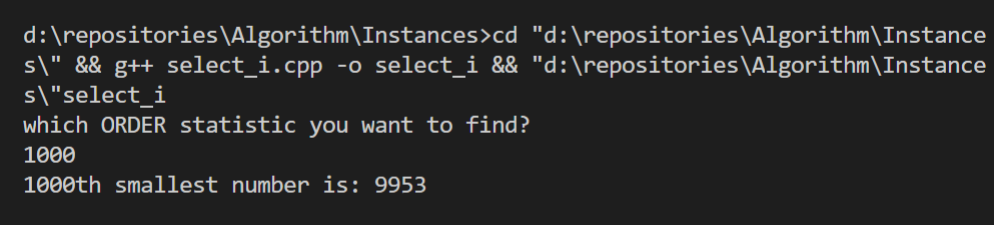
\includegraphics[width=12cm]{../Resources/6_1.png}
        \end{figure}
    经过验证(\emph{将A排序后输出A[999]}),结果正确。验证代码包含在源代码中(见注释)。
 
\end{document}